\documentclass[UTF8]{ctexart}

\usepackage{anyfontsize}
\usepackage{geometry}
    \geometry{left=4cm,right=4cm,top=2cm,bottom=2cm}
\usepackage{amsmath, amssymb, amsthm}
    \newtheorem{definition}{Definition}
    \newtheorem{theorem}{定理}
\usepackage{caption} 	 % 标题
\usepackage{xcolor} 	 % 颜色
\usepackage{graphicx} 	 % 引用图片
\usepackage{float}
\usepackage{framed} 	 % 方框 \begin{framed}
\usepackage{tcolorbox}
    \newtcolorbox{defbox}{colback = blue!20!green!10!white}
    \newtcolorbox{thmbox}{colback = black!5!white}
\usepackage{indentfirst} 	 % 首行缩进 
    \setlength{\parindent}{0em}
\usepackage{setspace} 	 % 行间距 \begin{spacing}{arg}
\usepackage{extarrows} 	 % 箭头宏包 \xLongrightarrow 
\usepackage{esvect} 	 % 向量箭头 \vv{}
\usepackage{siunitx} 	 % 国际单位 \si{unit} \SI{number}{unit} 
\usepackage{esint} 	 % 积分符号
\usepackage{mathrsfs}
\usepackage{mathtools}

% font
\newcommand{\ve}[1]{\boldsymbol{\mathbf{#1}}}
\newcommand{\unit}[1]{\boldsymbol{\mathbf{\hat{#1}}}}
\newcommand{\mr}{\mathrm}
\newcommand{\mcal}{\mathcal}
\newcommand{\mscr}{\mathscr}
% common symbol
\newcommand{\E}{\mathrm e}
\renewcommand{\I}{\mathrm i}
\newcommand{\R}{\mathbb R}
\newcommand{\Z}{\mathbb Z}
\newcommand{\N}{\mathbb N}
\newcommand{\Q}{\mathbb Q}
\newcommand{\C}{\mathbb C}
% differentiation
\def \DD #1.#2.#3 {\dfrac{d^{#1} #2}{d #3^{#1}}}
\def \PP #1.#2.#3 {\dfrac{\partial^{#1} #2}{\partial #3^{#1}}}
\def \dd #1.#2 {\dfrac{d #1}{d #2}}
\def \pp #1.#2 {\dfrac{\partial #1}{\partial #2}} 
\newcommand{\del}{\nabla}
% other
\newcommand{\transp}{^{\top}}
\DeclareMathOperator{\tr}{tr}
\pagestyle{empty}

\begin{document}
\section{基础知识}
\subsection{向量记法}
向量可以看作是有序 $ n- $元组, 亦可作为维度为 $ 1 \times n $ 或 $ m \times 1 $ 的行/列向量. 列向量比行向量更常用, 但两者本质是等价的.  约定本文中未经说明的向量, 默认为列向量. 下面的记法都是常见的.
\[ (v_1, v_2, \dots, v_n) \qquad \langle v_1, v_2, \dots, v_n \rangle \qquad \begin{bmatrix}
    v_1 \\ v_2 \\ \vdots \\ v_n
\end{bmatrix} \qquad   \]

\subsection{导数}
\subsubsection{标量对标量求导}
下面是常用的导数/偏导数记号:
\[ \dfrac{df}{dx} \equiv \dfrac{\partial f}{\partial x} \equiv f_x \equiv f'_x \equiv \partial_x f  \]

\subsubsection{向量对标量求导}
向量对标量求导, 即是对向量的每一个分量求导.
\vskip 1em
设 $ \ve{F} $ 为 $ \R^n $ 中的列向量, 其分量形式为 $ \ve{F} = \begin{bmatrix}
    F_1 & F_2 & \cdots & F_n
\end{bmatrix}\transp = \langle F_1, F_2, \dots, F_n \rangle $.
\[ \dfrac{\partial \ve{F}}{\partial t} = \ve{F}_t = \begin{bmatrix}
    \partial_t F_1 \\
    \partial_t F_2 \\
    \vdots \\
    \partial_t F_n 
\end{bmatrix} = \left\langle \dfrac{\partial F_1}{\partial t}, \dfrac{\partial F_2}{\partial t}, \dots, \dfrac{\partial F_n}{\partial t} \right\rangle \,.\]

\subsubsection{标量对向量求导}
向量对标量求导, 即是标量对向量的每一个分量求导, 并求转置. 向量在分母上结果就要求转置, 在分子上则直接求导, 不用转置. 这种叫做``分子布局'' (numerator layout).

\[ \dfrac{\partial y}{\partial \ve{x}} = \begin{bmatrix}
    \dfrac{\partial y}{\partial x_1} & \dfrac{\partial y}{\partial x_2} & \cdots & \dfrac{\partial y}{\partial x_n}
\end{bmatrix} \,.\]

\subsubsection{向量对向量求导}
$ \ve{y} $ 为 $ m $ 维向量, $ \ve{x} $ 为 $ n $ 维向量, $ \dfrac{\partial \ve{y}}{\partial \ve{x}} $ 为一个 $ m \times n $ 矩阵, 矩阵中 $ (i, j) $ 位置的元素为 $ \dfrac{\partial y_i}{\partial x_j} $, 所以有: 
\[ \dfrac{\partial \ve{y}}{\partial \ve{x}} = \Big[ \dfrac{\partial y_i}{\partial x_j} \Big]_{m \times n} = \begin{bmatrix}
    \dfrac{\partial y_1}{\partial x_1} & \dfrac{\partial y_1}{\partial x_2} & \cdots & \dfrac{\partial y_1}{\partial x_n} \\
    \dfrac{\partial y_2}{\partial x_1} & \dfrac{\partial y_2}{\partial x_2} & \cdots & \dfrac{\partial y_2}{\partial x_n} \\
    \vdots & \vdots & \ddots & \vdots \\
    \dfrac{\partial y_m}{\partial x_1} & \dfrac{\partial y_m}{\partial x_2} & \cdots & \dfrac{\partial y_m}{\partial x_n} 
\end{bmatrix} \,.\]





\section{Geometric Interpretation of Line Integral and Surface Integral}
\subsection{Preparation I}
Let $ \ve v \in \R^n $; $ \ve v $ can be expressed by its components: $\displaystyle \ve v = \sum_{i = 1}^n v_i \ve e_i $, where $ v_i $ and $ \ve e_i $ are respectively the $ i $-th component and $ i $-th base of $ \ve v $. Parameterize $ \ve v $ using $ t $:
\[ \ve v(t) = \sum_{i=1}^n v_i(t) \ve e_i \,,\]
\[ \ve v(t + \Delta t) = \sum_{i=1}^n v_i(t + \Delta t) \ve e_i \,,\]
\[ \Delta \ve v = \ve v(t + \Delta t) - \ve v(t) = \sum_{i=0}^{n} \big[ (v_i(t + \Delta t) - v_i(t)) \ve e_i \big] \,.\]

According to the mean value theorem, for $ 1 \leqslant i \leqslant n $, $ \exists t_i^* \in (t, t + \Delta t) $, such that: $ v_i (t + \Delta t) - v_i (t) = v_i'(t_i^*) \cdot \Delta t $. When $ \Delta t \to 0 $, $ t + \Delta t \to t $, $ t_i^* \to t $. Therefore
\[ \lim_{\Delta t \to 0} \big[  v_i (t + \Delta t) - v_i (t) \big] = v_i'(t) \Delta t \,,\]
\[ \lim_{\Delta t \to 0} \Delta \ve v = \sum_{i = 1}^n \big[ v_i'(t) \Delta t \cdot \ve e_i \big] = \sum_{i = 1}^n \big[ v_i'(t) \ve e_i \big]\cdot \Delta t = \ve v'(t) \Delta t \,. \tag{$ * $}\]

By convention, when $ \Delta t \to 0 $, it can be written in the form of $ dt $. 
\vskip 1em

\subsection{Line integral in scalar field}
The definition of line integral on scalar field:
\[ \int_C f(\ve r) \,ds \coloneqq \lim_{N \to \infty} \sum_{i = 1}^N f(\ve r_i) \Delta s_i \,.\]

Parameterize the curve using $ x = x(t), y = y(t), z = z(t), t \in [a, b] $, $ \ve r(x, y, z) $ now becomes $ \ve r(t) $. On the right-hand side, we have
\[ \lim_{\Delta t \to 0} \sum_{i = 1}^N f\big( \ve r(t) \big) \Delta s_i \,.\]

As we known from last section (equation $ * $), when $ \Delta t \to 0 $, $ \Delta s_i = |\ve r(t_i + \Delta t) - \ve r(t_i)| = |\ve r'(t_i)|\,dt $. So the integral
\[ \int_C f(\ve r)\, ds = \lim_{\Delta t \to 0} \sum_{i = 1}^N f\big( \ve r(t) \big) |\ve r'(t_i)|\Delta t_i = \int_a^b f\big(\ve r(t)\big)|\ve r'(t)|\,dt \,.\]


\subsection{Line integral on vector field}
The integral of $ \ve F(\ve r) $ along an oriented curve $ C \colon \ve r(t), t \in [a, b] $ is defined by:
\[ \int_C \ve F(\ve r) \cdot d \ve r \coloneqq \lim_{N \to \infty} \sum_{i = 1}^n \left[\ve F(\ve r_i) \cdot \Delta \ve r_i \right] \,.\]

Since $ N \to \infty $, $ \Delta \ve r \to \ve r'(t)\,dt $, therefore
\[ \lim_{N \to \infty} \sum_{i = 1}^n \big[ \ve F \big(\ve r(t_i)\big) \cdot \ve r'(t_i) \big] dt = \int_a^b \big[\ve F\big(\ve r(t)\big) \cdot \ve r'(t) \big]\,dt \,.\]

Here's another view: 
\[ \int_C \ve F(\ve r) \cdot d\ve r = \int_C \ve F(\ve r) \cdot \ve r'(t) \,dt = \int_C \ve F(\ve r) \cdot \unit{T} \,ds \,.\]

Since $ \unit{T} = \dfrac{\ve r'(t)}{|\ve r'(t)|} $ and $ ds = |\ve r'(t)| \,dt $, it's obvious that the second and third parts of the equation above are equivalent. It's common (especially in Physics) to see the notation $ d\ve\ell $ or $ d\ve s $. They are defined by $ d\ve\ell \equiv d\ve s \coloneqq \unit T \,ds $.


\subsection*{Preparation II}
Given a plane area $ A $, define $ \ve A \coloneqq |A| \ve n $. Here, $ |A| $ (or just $ A $) is the area of the plane, $ \ve n $ is the unit normal vector of the plane. $ \ve A $ or $ \ve B $ represents the area of the plane and the direction it towards.
\vskip 1em

Consider two area in space $ \ve A $ and $ \ve B $, $ \ve A \cdot \ve B = |A| |B| \ve n_{A} \cdot \ve n_B = |A| |B| \cos \theta $, where $ \theta $ is the angle between $ A $ and $ B $. So it's obvious that $ \cos \theta = \unit{A}\cdot \unit{B} $. The projection of $ A $'s area on $ B $ can be expressed as
\[ \operatorname{proj}_B A =  A_{\parallel B} = \ve A \cdot \unit B \,.\]

Note that $ \unit{B} $ stands for "unit vector in the same direction of $ \ve B $".
\vskip 1em
\subsection*{Surface integral on scalar field}
The definition of surface integral on a scalar field is given below:
\[ \iint_\Omega f(\ve r) \,dS \coloneqq \lim_{N \to \infty} \sum_{i = 1}^N f(\ve r_i) \Delta S_i \,.\]

Parameterize the surface:
\[
    \begin{cases}
        x = u \\
        y = v \\
        z = z(u, v)
    \end{cases}   \qquad \ve r(x, y, z) \Rightarrow \ve r\big(u, v, z(u, v)\big)
\,,\]

Consider a small patch $ \Delta \ve S $. $ \ve r_u \times \ve r_v $ is the normal vector of $ \Delta \ve S $. Denote $ \unit w = \unit u \times \unit v $, then the angle between $ \Delta S $ and $ Ouv $ is
\[ \cos \theta = \dfrac{(\ve r_u \times \ve r_v) \cdot \unit w}{|\ve r_u \times \ve r_v||\unit w|} \,.\]

$ \unit w = (0, 0, 1) $, $ |\unit w| = 1 $; $ \ve r_u = (1, 0, z_u) $, $ \ve r_v = (0, 1, z_v) $, so $ (\ve r_u \times \ve r_v) \cdot \unit w = \begin{vmatrix}
    1 & 0 & z_u \\
    0 & 1 & z_v \\
    0 & 0 & 1
\end{vmatrix} = 1 $.

\[ \cos \theta = \dfrac{1}{|\ve r_u \times \ve r_v|} \,.\]

$ \Delta S \cdot \cos\theta = \Delta S_{uv} = \Delta A $, we have
\begin{align*}
    \iint_\Omega f(\ve r) \,dS &= \lim_{N \to \infty} \sum_{i = 1}^N f(\ve r_i) \Delta S_i \\
    &= \lim_{N \to \infty} \sum_{i = 1}^N \ve F\big(\ve r(u_i, v_i)\big)\cdot \dfrac{\Delta A}{\cos \theta} \\
    &= \lim_{N \to \infty} \sum_{i = 1}^N \ve F\big(\ve r(u_i, v_i)\big) |\ve r_u \times \ve r_v| \Delta A \\
    &= \iint_{\Omega_{uv}} \ve F(\ve r(u, v)) |\ve r_u \times \ve r_v| \,du\,dv
\end{align*} 


\subsection{Surface integral on vector field}
The definition of surface integral on a vector field is given below. Note that $ \Delta \ve S = \Delta S \cdot \unit n $, in which $ \unit n $ is the unit normal vector of area $ \Delta S $. With the conclution we got from last section: $ \cos \theta = |\ve r_u \times \ve r_v|^{-1} $, $ \theta $ means the angle between $ \Delta S $ and $ \Delta A $.
\begin{align*}
    \iint_{\ve\Omega} \ve F(\ve r) \cdot d\ve S &= \lim_{N \to \infty} \sum_{i = 1}^N \ve F(\ve r_i) \cdot \Delta \ve S_i \\
    &= \lim_{N \to \infty} \sum_{i = 1}^N \ve F(\ve r_i) \cdot \unit n \,\Delta S_i \\
    &= \lim_{N \to \infty} \sum_{i = 1}^N \ve F(\ve r_i) \cdot \dfrac{\ve r_u \times \ve r_v}{|\ve r_u \times \ve r_v|} \,\Delta S_i \\
    &= \lim_{N \to \infty} \sum_{i = 1}^N \ve F(\ve r_i) \cdot \dfrac{\ve r_u \times \ve r_v}{|\ve r_u \times \ve r_v|} \,\dfrac{\Delta A_i}{\cos\theta} \\
    &= \lim_{N \to \infty} \sum_{i = 1}^N \ve F(\ve r_i) \cdot (\ve r_u \times \ve r_v) \,\Delta A_i \\
    &= \iint_{\ve\Omega_{uv}} \ve F(\ve r(u, v)) \cdot (\ve r_u \times r_v) \,du\,dv
\end{align*}
Here, $ \ve r_u = \pp {\ve r}.{u} $, $ \ve r_v = \pp {\ve r}.{v} $.




\section{曲线积分和曲面积分计算}
\subsection{曲线积分}
\subsubsection{标量场}
设标量场 $ f(\ve{r}): \R^3 \to \R $ 中有一条参数化曲线 $ \gamma: \ve{r} (t), t \in [a, b] $. 则沿该曲线积分的计算如下:
\begin{thmbox}
    \[ \int_\gamma f(\ve{r}) \,ds = \int_{a}^{b} f\big( \ve{r}(t) \big) |\ve{r}'(t)|\,dt  \,.\]
\end{thmbox}

\subsubsection{向量场}
设向量场 $ \ve{F}(\ve{r}) : \R^3 \to \R^3 $ 中有一条定向曲线 $ \ve{\gamma}: \ve{r}(t), t \in [a, b] $. 则沿该曲线积分得到标量:
\begin{thmbox}
    \[ \int_{\ve{\gamma}} \ve{F} (\ve{r}) \cdot d\ve{s} = \int_{a}^{b} \ve{F} \big( \ve{r} (t) \big) \cdot \ve{r}'(t) \,dt \,.\]
\end{thmbox} 

使用微分形式计算, 
\begin{thmbox}
    \begin{align*}
        \int_{\ve{\gamma}} \ve{F} (\ve{r}) \cdot d\ve{s} &= \int_{\ve{\gamma}} F_1 \,dx + F_2 \,dy + F_3 \,dz \\ 
        &= \int_{a}^{b} F_1 \big( \ve{r} (t) \big) \, dx(t) + F_2 \big( \ve{r} (t) \big) \, dy(t) + F_3 \big( \ve{r} (t) \big) \, dz(t) \\
        &= \int_{a}^{b} (F_{1t} x_t + F_{2t} y_t + F_{3t} z_t) \,dt
    \end{align*}
\end{thmbox}

此处, $ x_t = \dfrac{\partial x}{\partial t} $, $ y_t = \dfrac{\partial y}{\partial t} $, $ z_t = \dfrac{\partial z}{\partial t} $; $ F_{it} $ 表示参数化, 即 $ F_{it} = F_i \big( \ve{r} (t) \big) $.

\subsection{曲面积分}
\subsubsection{标量场}
标量场 $ f (\ve{r}) : \R^3 \to \R $ 中有一个参数化曲面 $ \Omega: \ve{r}\big( x(u, v), y(u, v), z(u, v) \big) $. 这个曲面上的积分计算方法如下:
\begin{thmbox}
    \[ \iint_\Omega f(\ve{r}) \,dS = \iint_{\Omega_{uv}} f\big( \ve{r}(u, v) \big) \left| \dfrac{\partial \ve{r}}{\partial u} \times \dfrac{\partial \ve{r}}{\partial v} \right| \,du\,dv \]
\end{thmbox}

\subsubsection{向量场}
向量场 $ \ve{F} (\ve{r}) : \R^3 \to \R^3 $ 中有一个可定向曲面 $ \ve{\Omega}: \ve{r}\big( x(u, v), y(u, v), z(u, v) \big) $. 这个曲面上的积分方法如下:
\begin{thmbox}
    \[ \iint_{\ve{\Omega}} \ve{F} (\ve{r}) \cdot \ve{S} = \iint_{\ve{\Omega}_{uv}} \ve{F} \big( \ve{r} (u, v) \big) \cdot \left( \dfrac{\partial \ve{r}}{\partial u} \times \dfrac{\partial \ve{r}}{\partial v} \right) \,du\,dv \,.\]
\end{thmbox}

记 $ \ve{F} $ 参数化后, 各分量为: $ P = F_1 \big( \ve{r}(u, v) \big) $, $ Q = F_2 \big( \ve{r}(u, v) \big) $, $ R $ 同理. $ \ve{r} = \langle x, y, z \rangle $, 参数化后, $ \ve{r}(u, v) = \langle x(u, v), y(u, v), z(u, v) \rangle $. $ \ve{r}_u = \langle x_u, y_u, z_u \rangle $, $ \ve{r}_v = \langle x_v, y_v, z_v \rangle $. 由标量三重积的性质, 上面的计算公式可以等价为:
\[ \iint_{\ve{\Omega}_{uv}} \ve{F} \big( \ve{r} (u, v) \big) \cdot \left( \dfrac{\partial \ve{r}}{\partial u} \times \dfrac{\partial \ve{r}}{\partial v} \right) \,du\,dv = \iint_{\ve{\Omega}_{uv}} \begin{vmatrix}
    P & Q & R \\
    x_u & y_u & z_u \\
    x_v & y_v & z_v
\end{vmatrix} \,du\,dv \tag{$ * $}\]

使用微分形式计算向量场中的曲面积分, 注意楔积性质 $ dx \land dy = - dy \land dx $ 以及 $ dx \land dx = 0 $, 同时使用全微分公式 $ dx = x_u\,du + x_v \,dv $. 
\begin{thmbox}
    \[ \iint_{\ve{\Omega}} \ve{F} (\ve{r}) \cdot \ve{S} = \iint_{\ve{\Omega}} {\color{red} F_1 \,dy\land dz} + {\color{blue} F_2 \,dz \land dx} + {\color{olive} F_3 \,dx \land dy} \,,\]
\end{thmbox}

参数化后:
\begin{align*}
    F_1 \,dy \land dz &= P \, (y_u \,du + y_v \,dv) \land (z_u \,du + z_v \, dv) \\
    &= P (y_u z_u \,du \land du + y_u z_v \,du\land dv + y_v z_u \, dv \land du + y_v z_v \,dv \land dv ) \\
    &= P (y_u z_v \,du \land dv + y_v z_u \,dv \land du) 
    = P (y_u z_v \,du \land dv - y_v z_u \,du \land dv) \\
    &= P \begin{vmatrix}
        y_u & z_u \\
        y_v & z_v 
    \end{vmatrix} \,du \land \,dv \,,
\end{align*}

同理: 
\[ F_2 \, dz \land dx = Q \begin{vmatrix}
    z_u & x_u \\
    z_v & x_v
\end{vmatrix} \, du \land dv \,,\]
\[ F_3 \,dx \land dy = R \begin{vmatrix}
    x_u & y_u \\
    x_v & y_v
\end{vmatrix} \, du \land dv \]

将三项相加, 即得到 $ (*) $ 式.

\section{梯度, 散度和旋度}
\subsection{等高线与水平曲面}
对于二元函数, $ f(x, y) $ 和常数 $ c $, $ f(x, y) = c $ 的曲线被称为该二元函数的等高线 (contour line). 同理, 三元函数取常数 $ f(x, y, z) = c $ 时获得的曲面被称为水平曲面 (level surface) 或等值曲面 (isosurface).

\subsection{梯度}
设 $ f(x, y, z): \R^3 \to \R $. 记 $ \del f = \left( \dfrac{\partial f}{\partial x}, \dfrac{\partial f}{\partial y}, \dfrac{\partial f}{\partial z} \right) = \dfrac{\partial f}{\partial x} \ve{i} + \dfrac{\partial f}{\partial y} \ve{j} + \dfrac{\partial f}{\partial z} \ve{k} $. 也即: $ \del = \dfrac{\partial  }{\partial x} \ve{i} + \dfrac{\partial  }{\partial y} \ve{j} + \dfrac{\partial  }{\partial z} \ve{k} $.
\vskip 1em

对于空间中的函数 $  f(x, y, z) $, $ \del f $ 是一个 $ \R^3 $ 向量场. 且 $ \del f $ 是水平曲面 $ f(x, y, z) = c $ 的法向量. $ \del f $ 指向函数值增加最快的方向; 梯度的大小为该方向的增长率, 即最大``斜率''.
\vskip 1em 

\begin{figure}[H]
    \centering
    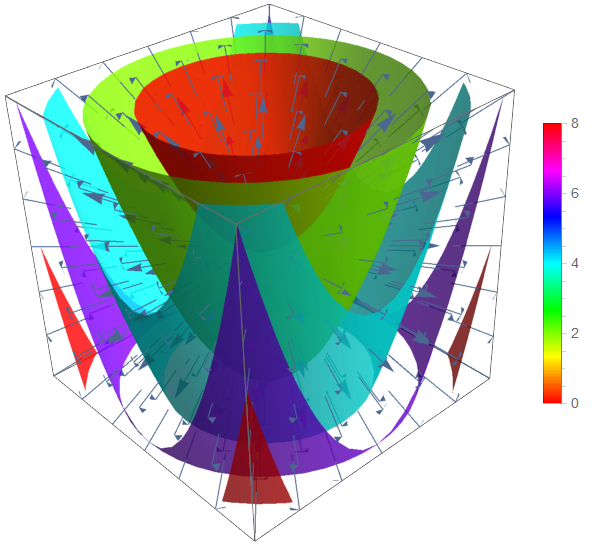
\includegraphics[width = 0.5\linewidth]{./pic/grad_3d.png}
\end{figure}


对于平面内的二元函数 $ f(x, y) $, $ \del f = \left( \dfrac{\partial f}{\partial x}, \dfrac{\partial f}{\partial y} \right) $ 是一个平面向量场, 是等高线的法向量, 且指向函数值增加最快的方向; 梯度的大小也为该方向的增长率, 即最大斜率.

\begin{figure}[H]
    \centering
    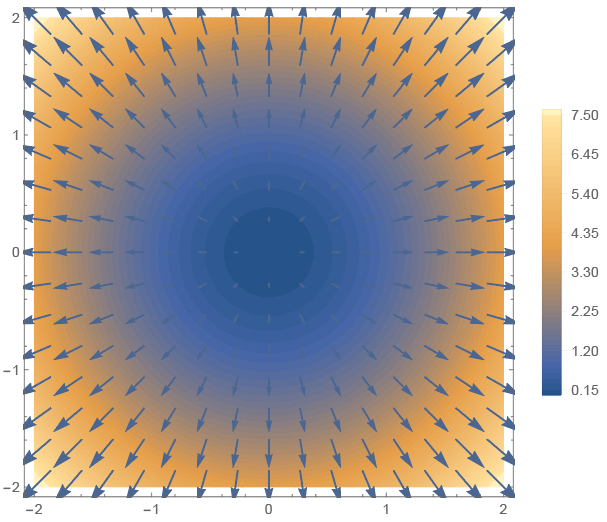
\includegraphics[width = 0.54\linewidth]{./pic/grad_2d.png}
\end{figure}

\subsubsection{方向导数}
借助梯度, 可以计算 $ f: \R^n \to \R $ 在任意方向 $ \ve{v} $ 的导数 $ D_{\ve{v}} $.
\[ D_{\ve{v}} f = \del f \cdot \unit v \,.\]

如果 $ \ve{v} $ 指向变化率最大的方向, 即和 $ \del f $ 同向, 则计算得到 $ D_{\ve{v}} f = \del f $. 反向, 即函数值下降最快的方向, 则得到 $ D_{\ve{v}} f = - \del f $.
\vskip 1em

举例: 一元函数 $ f(x) $ 只有一个走向, $ x $ 轴正向, 此处 $ \ve{v} $ 即沿 $ x $ 轴正向. 梯度 $ \del f = \dfrac{\partial f}{\partial x} \ve{i} = \dfrac{\partial f}{\partial x} \unit x $. 当函数上升时, 梯度方向 $ \del f $ 和 $ \ve{v} $ 方向一致, 所以方向导数 $ D_{\ve{v}} f = \dfrac{\partial f}{\partial x} \ve{i} = \dfrac{\partial f}{\partial x} = \dfrac{df}{dx} $. 当函数下降时, 梯度方向和所求导数方向相反, 方向导数 $ D_{\ve{v}} f = - \del f = - \dfrac{df}{dx} $. 
\begin{figure}[H]
    \centering
    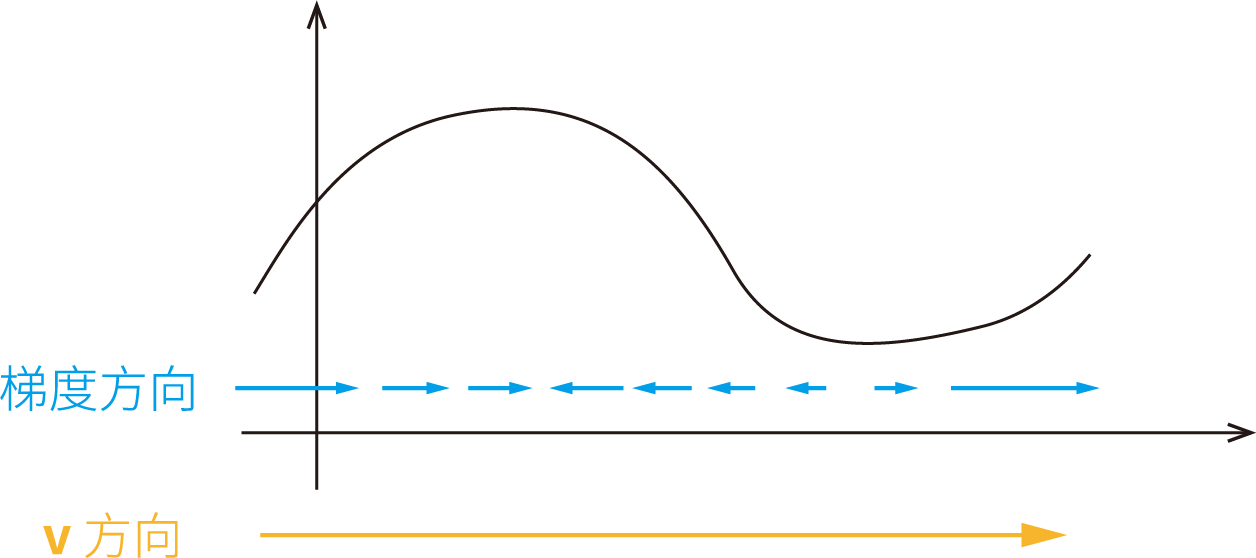
\includegraphics[width = 0.6\linewidth]{./pic/example_1d.png}
\end{figure}


\subsubsection{柱坐标系中的梯度算子}
\[ \del_{(r, \varphi, z)} = \left( \dfrac{\partial}{\partial r},\ \dfrac{1}{r} \dfrac{\partial}{\partial \varphi},\ \dfrac{\partial}{\partial z} \right) = \left( \partial_r, \dfrac{\partial_\varphi}{r}, \partial_z \right) \]

\subsubsection{球坐标系中的梯度算子}
\[ \del_{(r, \theta, \varphi)} = \left( \dfrac{\partial}{\partial r},\ \dfrac{1}{r} \dfrac{\partial}{\partial \theta},\ \dfrac{1}{r \sin \theta} \dfrac{\partial}{\partial \varphi} \right) = \left( \partial_r, \dfrac{\partial_\theta}{r}, \dfrac{\partial_\varphi}{r \sin\theta} \right) \]



\subsubsection{梯度定理}
梯度定理是微积分基本定理在曲线积分中的推广. 

\begin{thmbox}
    \begin{theorem}
        设有 $ \R^n $ 标量场 $ f $ 和其梯度场 $ \del f $. 则任意一条以点 $ \ve{p} $ 为起点, $ \ve{q} $ 为终点的曲线 $ \gamma[\ve{p}, \ve{q}] $ 上梯度场的积分都是固定的, 即积分与路径无关. 满足这种性质的场, 便称为保守场.
        \[ \int_{\ve{\gamma}[\ve{p}, \ve{q}]} \del f \cdot d\ve{r} = \big[ f(\ve{r}) \big]_{\ve{p}}^{\ve{q}} = f(\ve{q}) - f(\ve{p})  \,.\]
    \end{theorem} 
\end{thmbox}
\begin{figure}[H]
    \centering
    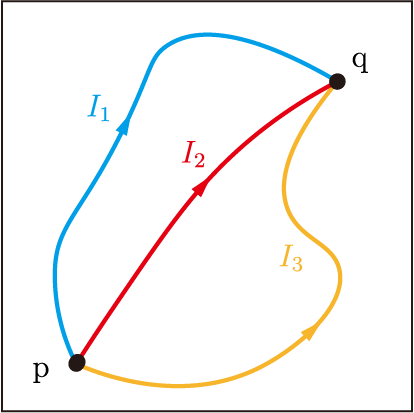
\includegraphics[width = 0.4\linewidth]{./pic/gradient_thm.png}
    \caption{梯度定理: 积分与路径无关, $ I_1 = I_2 = I_3 $}
\end{figure}





\end{document}